\documentclass[12pt,a4paper]{article}
\usepackage[utf8]{inputenc}
\usepackage[T1]{fontenc}
\usepackage[spanish,es-tabla]{babel}
\usepackage[margin=2.5cm]{geometry}
\usepackage{graphicx,longtable,array,xcolor,listings,hyperref}
\usepackage{setspace}
\setstretch{1.15}
\hypersetup{colorlinks=true,linkcolor=blue,urlcolor=blue}
\setlength{\emergencystretch}{3em}
\lstset{basicstyle=\ttfamily\scriptsize,breaklines=true,columns=fullflexible,keepspaces=true,showstringspaces=false,frame=single,inputencoding=utf8,literate={á}{{\'a}}1 {é}{{\'e}}1 {í}{{\'i}}1 {ó}{{\'o}}1 {ú}{{\'u}}1 {ñ}{{\~n}}1 {Á}{{\'A}}1 {É}{{\'E}}1 {Í}{{\'I}}1 {Ó}{{\'O}}1 {Ú}{{\'U}}1 {Ñ}{{\~N}}1 {ü}{{\"u}}1 {–}{{-}}1 {·}{{$\cdot$}}1 {→}{{$\rightarrow$}}1 {«}{{\guillemotleft}}1 {»}{{\guillemotright}}1}
\newcommand{\codigo}[1]{\texttt{\detokenize{#1}}}
\begin{document}
\begin{titlepage}
\centering
{\Large INFORME TÉCNICO DE DESARROLLO DE LA INTERFAZ DE USUARIO (UI/UX)\par}
\vspace{1.5cm}
{\LARGE\bfseries Resumen semanal de hábitos de estudio y bienestar\par}
\vspace{1.5cm}
\begin{tabular}{p{3.4cm}p{9cm}}
Asignatura: & Desarrollo de Software II (IF616BIN)\\[0.4cm]
Unidad: & I -- Fundamentos de Dart, UI declarativa y UX\\[0.4cm]
Proyecto: & Resumen semanal de hábitos de estudio y bienestar\\[0.4cm]
Integrantes: & [Completar apellidos y nombres]\\[0.4cm]
Fecha: & 6 de octubre de 2026 (fecha de elaboración; confirmar entrega)\\[0.4cm]
URL GitHub: & No identificada en los archivos revisados. Código incluido en el Anexo A.
\end{tabular}
\vfill
\begin{flushleft}
\textbf{Base del informe.} Revisión del proyecto ubicado en \codigo{E:\desII}, sus archivos fuente, documentación, pruebas y capturas existentes. El esquema proporcionado determina la estructura; los ejemplos de ese esquema no se presentan como características implementadas. Los datos personales y la fecha de entrega definitiva requieren completar la portada.
\end{flushleft}
\end{titlepage}
\tableofcontents
\newpage
\section{Introducción y Objetivos}
\subsection{Descripción del Proyecto}
La aplicación es una demostración académica de una única pantalla desarrollada con Flutter y Dart. Presenta un resumen de hábitos de estudio y bienestar para un usuario de ejemplo llamado Alex. Su contenido integra un saludo, calendario de siete días, cuatro métricas, dos indicadores de progreso, una tarjeta de logro y tres recordatorios. La interfaz permite consultar información relacionada sin cambiar de pantalla.

La fecha visible es martes 6 de octubre de 2026 y la semana resumida corresponde al 28 de septiembre al 4 de octubre de 2026. Esta distinción se comunica mediante la etiqueta ``Semana resumida anterior''. Los valores son datos de demostración: 18 horas de estudio, 7,5 horas de sueño por noche, 180 minutos de actividad física y 82\% de cumplimiento de metas. El calendario muestra cinco días cumplidos y dos pendientes; el 82\% es un dato independiente suministrado, no el porcentaje de esos siete días.
\subsection{Objetivo de la Interfaz}
El objetivo general es presentar el resumen semanal de forma legible, organizada y adaptable a distintos tamaños de pantalla. Los objetivos específicos son componer widgets reutilizables; establecer una jerarquía visual entre títulos, valores y descripciones; conservar el contenido con texto ampliado; evitar desbordamientos mediante restricciones finitas y distribuciones flexibles; y aportar información semántica a estados e indicadores relevantes.
\subsection{Alcance de la Sesión}
La entrega corresponde exclusivamente a UI estática. Todos los widgets propios extienden \codigo{StatelessWidget}. No existen navegación, llamadas a servicios, base de datos, persistencia, gestores de estado ni actualización funcional de hábitos. Los cálculos de ancho y las decisiones según restricciones pertenecen al layout, no a lógica de negocio. Los recordatorios son textos informativos y no programan notificaciones. La configuración interna de los widgets del SDK no altera este alcance.
\section{Arquitectura de Widgets y Estructura del Código}
\subsection{Organización del Proyecto}
\begin{lstlisting}
lib/
  main.dart
  screens/weekly_summary_screen.dart
  widgets/header_section.dart
  widgets/weekly_calendar.dart
  widgets/metric_card.dart
  widgets/progress_summary.dart
  widgets/achievement_card.dart
  widgets/reminder_card.dart
  utils/app_constants.dart
test/weekly_summary_screen_test.dart
android/                    configuracion Android
web/                        configuracion web
pubspec.yaml                dependencias y configuracion
analysis_options.yaml       reglas de analisis
README.md                   ejecucion y decisiones de layout
DEEPSEEK_TASK.md             especificacion previa
build/                      productos generados y capturas
.dart_tool/                 archivos de herramientas
.idea/                      configuracion del entorno
\end{lstlisting}
\codigo{main.dart} inicia la aplicación y configura Material 3. La carpeta \codigo{screens} compone la pantalla; \codigo{widgets} contiene bloques visuales; \codigo{utils} concentra colores, tipografía, espaciados y datos mock. Los tipos inmutables \codigo{StudyDay}, \codigo{WeeklyMetric} y \codigo{StudyReminder} permanecen junto a las constantes porque solo transportan datos estáticos. No se necesitan capas de servicios o repositorios.

Esta separación facilita localizar decisiones visuales y evita repetir el diseño de tarjetas. Por ejemplo, \codigo{MetricCard} recibe parámetros finales y sirve para las cuatro métricas. \codigo{_ProgressCard} comparte la presentación y semántica de los dos indicadores. Los archivos generados de plataforma y herramientas no constituyen componentes de la arquitectura visual. \codigo{DEEPSEEK_TASK.md} describe una tarea anterior; sus instrucciones no se ejecutan como parte de la redacción de este informe.

En \codigo{pubspec.yaml} solo se declara Flutter como dependencia de ejecución y \codigo{flutter_test} y \codigo{flutter_lints} como dependencias de desarrollo. El requisito de Dart es \codigo{^3.11.5}; el README documenta Flutter 3.41.x. Estas referencias describen la configuración registrada y no sustituyen una comprobación de versión ejecutada.
\subsection{Árbol de Widgets Principal (Blueprint)}
\begin{lstlisting}
ResumenSemanalApp (StatelessWidget)
  MaterialApp (Material 3)
    WeeklySummaryScreen
      Scaffold
        SafeArea
          SingleChildScrollView
            Center
              ConstrainedBox (maxWidth: 1120)
                Padding
                  LayoutBuilder
                    Column (mainAxisSize: min)
                      HeaderSection (Row / Expanded / CircleAvatar)
                      Text: Tu resumen semanal
                      WeeklyCalendar (LayoutBuilder / Row o Wrap)
                      _MetricsSection (LayoutBuilder / Wrap)
                        4 MetricCard
                      ProgressSummary (LayoutBuilder / Row o Column)
                        _LinearProgressBlock
                        _CircularProgressBlock
                      AchievementCard (Stack / Positioned)
                      _RemindersSection
                        ListView.separated
                          3 ReminderCard
\end{lstlisting}
\codigo{Column} expresa el orden de lectura vertical; \codigo{SingleChildScrollView} permite recorrer el contenido cuando supera la altura disponible. \codigo{Center} y \codigo{ConstrainedBox} mantienen una composición centrada sin estirar las tarjetas indefinidamente en escritorio. \codigo{SafeArea} protege el contenido frente a áreas reservadas del dispositivo. Los \codigo{LayoutBuilder} internos resuelven la distribución con el ancho realmente asignado a cada sección. El \codigo{LayoutBuilder} exterior recibe restricciones, aunque su parámetro no se utiliza para decidir la distribución; las adaptaciones efectivas se realizan en los bloques internos.
\section{Implementación de Widgets Clave y Decisiones de Diseño}
\subsection{Widgets de Contenido (Text, Image, Icon)}
La jerarquía tipográfica está centralizada en \codigo{AppTypography}: título principal de 28 sp, títulos de sección de 20 sp, valores de métricas de 30 sp, cuerpo de 16 sp y texto secundario de 14 sp. \codigo{AppTextStyles} combina estos tamaños con pesos de 600 y 700 para destacar encabezados y cifras. Las alturas de línea de 1,1 a 1,3 favorecen una lectura compacta sin fijar la altura de las tarjetas.

El código no utiliza \codigo{maxLines} ni \codigo{TextOverflow.ellipsis}. En esta pantalla se preserva la información completa mediante salto de línea y altura natural; \codigo{Expanded} y \codigo{Flexible} limitan el ancho del texto donde corresponde. El nombre ``Cumplimiento de metas'' puede ocupar varias líneas en móvil. Si en el futuro se requiere limitar títulos, debe evaluarse el truncamiento sin ocultar datos esenciales.

No hay \codigo{Image.network} ni \codigo{Image.asset} en los widgets de la aplicación; por ello \codigo{BoxFit.cover} y \codigo{BoxFit.contain} no son decisiones aplicadas. Se emplean iconos Material incluidos en Flutter y un \codigo{CircleAvatar} con la inicial A. Esto evita dependencias de imágenes y mantiene el alcance estático. Los iconos de lanzamiento presentes en Android y web son recursos de plataforma, no imágenes del contenido.

La insignia de trofeo declara \codigo{semanticLabel: MockData.achievementBadgeSemantics}. Calendario, avatar y progreso usan \codigo{Semantics} con etiquetas explícitas. En esos grupos, \codigo{excludeSemantics: true} evita repetir los hijos en el anuncio. No todos los iconos decorativos tienen exclusión semántica explícita; no se debe confundir la intención documentada con una auditoría completa mediante lector de pantalla.
\subsection{Modelo de Caja (Padding, Margin, Container)}
La escala de espaciado es 4, 8, 12, 16, 24 y 32 dp, con una unidad mínima de 4 dp. El padding común de tarjeta es 16 dp, la separación de métricas 12 dp y la separación de secciones 24 dp. Los radios son 16 dp para tarjetas, 12 dp para celdas y 8 dp para indicadores.

\codigo{EdgeInsets.all(16)} separa el contenido del borde de las tarjetas. \codigo{EdgeInsets.symmetric} aplica padding exterior horizontal de 16 o 24 dp y vertical de 24 dp. \codigo{EdgeInsets.fromLTRB} reserva en el logro 16 dp a la izquierda, 24 arriba, 56 a la derecha y 16 abajo para proteger el texto frente al trofeo. \codigo{EdgeInsets.only} no se emplea en esta implementación.

El padding es separación interna; el margin es separación externa. \codigo{ReminderCard} declara \codigo{margin: EdgeInsets.zero}, mientras los separadores de la lista aportan 12 dp entre tarjetas. Secciones y elementos también se separan con \codigo{SizedBox}; no se atribuyen esos espacios a un margin inexistente.

\codigo{BoxDecoration} define fondos suaves, bordes y esquinas redondeadas. No se utiliza \codigo{boxShadow}; los recordatorios tienen elevación cero. En un \codigo{Container} decorado, el color se declara dentro de la decoración; declarar simultáneamente \codigo{color} y \codigo{decoration} en ese mismo contenedor sería incompatible. El código revisado mantiene esa separación.
\subsection{Layout Flexible (Row, Column, Expanded, Flexible)}
En la cabecera, \codigo{Expanded} asigna al saludo y fecha el espacio restante después de reservar el avatar y su separación. En el calendario amplio reparte el ancho entre siete celdas. En el progreso amplio divide el espacio entre dos bloques y en los recordatorios permite ajustar el nombre sin desplazar la hora fuera de la tarjeta.

\codigo{Flexible} se usa para la unidad de cada métrica: puede ocupar menos que el espacio asignado o envolver su texto, mientras la cifra conserva protagonismo. La diferencia práctica es que \codigo{Expanded} exige ocupar el espacio restante asignado y \codigo{Flexible} admite una ocupación menor. No se declaran valores \codigo{flex} personalizados: el reparto de los \codigo{Expanded} hermanos utiliza el valor predeterminado 1; no existe un reparto 2:1.

\codigo{crossAxisAlignment.start} alinea textos a la izquierda y bloques de una fila por su borde superior. La columna principal utiliza \codigo{crossAxisAlignment.stretch} para ocupar el ancho permitido. La fila de valor y unidad usa alineación por línea base con \codigo{TextBaseline.alphabetic}. Los recordatorios y el indicador circular alinean sus elementos al centro vertical. Al no declararse otro \codigo{mainAxisAlignment}, se conserva el inicio del eje principal; los huecos se controlan con separadores explícitos.
\subsection{Superposición y Flujo (Stack, Wrap)}
\codigo{AchievementCard} utiliza \codigo{Stack} y \codigo{Positioned(top: 0, right: 0)} para situar una insignia circular de 44 por 44 dp. El espacio reservado evita que el trofeo cubra el título. El código no configura \codigo{clipBehavior}, por lo que mantiene el comportamiento predeterminado \codigo{Clip.hardEdge}; no necesita \codigo{Clip.none} porque la insignia se ubica dentro de sus límites.

\codigo{Wrap} permite redistribuir las métricas y los días sin imponer una única fila en pantallas pequeñas. En métricas, \codigo{spacing} y \codigo{runSpacing} valen 12 dp; en el calendario, 8 dp. El estado de cada día usa otro \codigo{Wrap} con separación de 4 dp, de modo que el icono y la palabra pueden cambiar de renglón. Los hijos principales tienen un ancho finito calculado; no se coloca \codigo{Expanded} directamente dentro de un \codigo{Wrap}.
\section{Adaptabilidad y Prevención de Errores de Layout}
\subsection{Diseño Adaptativo (LayoutBuilder, MediaQuery)}
\codigo{MediaQuery} proporciona el tamaño global y el escalado de texto. \codigo{LayoutBuilder} aporta el ancho local después del límite máximo y del padding. Por esa razón un breakpoint local no equivale al ancho total de la ventana.
\begin{longtable}{p{3cm}p{10.5cm}}
\textbf{Bloque} & \textbf{Regla implementada}\\\hline
Exterior & Viewport menor de 600 dp: padding horizontal 16 dp; desde 600: 24 dp. Contenido limitado a 1120 dp antes del padding.\\
Métricas & Ancho local desde 900 dp y texto normal: cuatro columnas. Menos de 900: dos; menos de 280 o texto grande: una. Separación: 12 dp.\\
Calendario & Desde 700 dp locales y texto normal: siete celdas con Expanded. En otro caso Wrap con ancho mínimo aproximado 96 dp por celda, o 128 dp con texto grande.\\
Progreso & Desde 600 dp locales y texto normal: dos bloques en Row; en otro caso Column.\\
Recordatorios & Menos de 360 dp locales o texto grande: la hora aparece debajo del nombre.\\
Texto grande & Se detecta cuando el escalado de un texto de 16 sp supera 20 sp. No se desactiva el escalado del sistema.\\\hline
\end{longtable}
Para las métricas, el ancho de tarjeta es $w=(W-12(n-1))/n$, donde $W$ es el ancho local y $n$ el número de columnas. Con viewport de 390 dp, $W=358$ y cada tarjeta mide 173 dp; con 1280 dp, el límite de 1120 y padding de 48 dejan $W=1072$, por lo que cada tarjeta mide 259 dp. En el calendario se calcula el número de columnas mediante el ancho disponible, separación de 8 dp y ancho mínimo de celda, acotándolo entre uno y siete.

No se encontró un panel de diagnóstico implementado. Existe una suite con 16 pruebas: tres de composición, dos de progreso, dos de accesibilidad, seis de layout y tres de distribución de métricas. Contempla tamaños 320 por 800, 390 por 844, 768 por 1024 y 1280 por 900, además de texto al 200\% en móvil y escritorio. La revisión confirma que las pruebas están escritas; su ejecución durante esta elaboración no devolvió un resultado verificable, por lo que no se afirma que hayan pasado.
\subsection{Prevención de Errores (Overflow, Constraints)}
La prevención de \codigo{RenderFlex overflowed} se apoya en limitar el texto de las filas con \codigo{Expanded} o \codigo{Flexible}, permitir saltos de línea, cambiar distribuciones y evitar alturas fijas en tarjetas. El indicador circular sí tiene una caja finita de 80 por 80 dp; su porcentaje se muestra fuera del círculo, evitando que el escalado tipográfico lo recorte dentro de esa caja.

El scroll exterior proporciona altura no acotada al contenido. La columna usa \codigo{mainAxisSize: MainAxisSize.min} y no contiene flexibles verticales que intenten consumir una altura infinita. La lista corta de recordatorios declara \codigo{shrinkWrap: true}, \codigo{primary: false} y \codigo{NeverScrollableScrollPhysics}; calcula su altura por contenido y delega el desplazamiento a la página. Los \codigo{Expanded} existentes pertenecen a filas con ancho limitado.

No se identificó evidencia de una sesión de Flutter Inspector ni una activación de \codigo{debugPaintSizeEnabled}. Las capturas y el código permiten revisar la composición, pero no acreditan esa verificación solicitada por el esquema. Para completar esa evidencia debe registrarse una revisión con Inspector y conservar su captura.
\subsection{Accesibilidad y UX}
La pantalla evita comunicar estados solo mediante color: los días incluyen ``Cumplido'' o ``Pendiente'' y un icono correspondiente. El avatar anuncia ``Perfil de ejemplo''; los bloques de progreso aportan etiqueta y valor ``82\%''. El porcentaje también es visible, y las tarjetas crecen cuando el texto necesita más líneas.

Los textos principales oscuros sobre fondos claros y los fondos suaves permiten diferenciar jerarquías sin recargar la interfaz. Esta observación visual no equivale a una medición formal de contraste ni a una certificación de accesibilidad. Se recomienda medir los pares efectivos de texto y fondo y realizar una prueba con lector de pantalla.

No hay controles interactivos: el avatar mide 48 dp de diámetro pero no es un botón. Los iconos de métricas y el trofeo son informativos. En consecuencia, no corresponde afirmar que se verificaron zonas táctiles de 48 por 48 dp para acciones inexistentes. Al incorporar acciones futuras habrá que asegurar ese tamaño mínimo en sus áreas de toque.
\section{Resultados y Evidencias}
\subsection{Capturas de Pantalla}
Se localizaron cinco imágenes en \codigo{build/shots}: \codigo{mobile_390.png}, \codigo{mobile_iframe_390.png}, \codigo{mobile390_css.png}, \codigo{mid_768.png} y \codigo{wide_1280.png}. Se seleccionan la vista móvil contenida en \codigo{mobile_iframe_390.png} y la vista amplia \codigo{wide_1280.png}, revisadas visualmente. Son evidencias preexistentes y no capturas de una ejecución nueva durante la elaboración.

La vista móvil seleccionada muestra el avatar completo, el calendario en varias filas, dos columnas de métricas, progreso vertical y las horas debajo del nombre de los recordatorios. La imagen contiene margen externo a la derecha: el viewport de la aplicación corresponde a la franja móvil identificada por el archivo. La vista amplia muestra los siete días en una fila, cuatro métricas y dos bloques de progreso lado a lado. El archivo alternativo \codigo{mobile_390.png} presenta contenido cortado por la derecha y no se usa como prueba concluyente de adaptación correcta; sin conocer su método de captura no puede atribuirse automáticamente ese recorte al código actual.
\begin{figure}[htbp]
\centering
\IfFileExists{vista_movil.png}{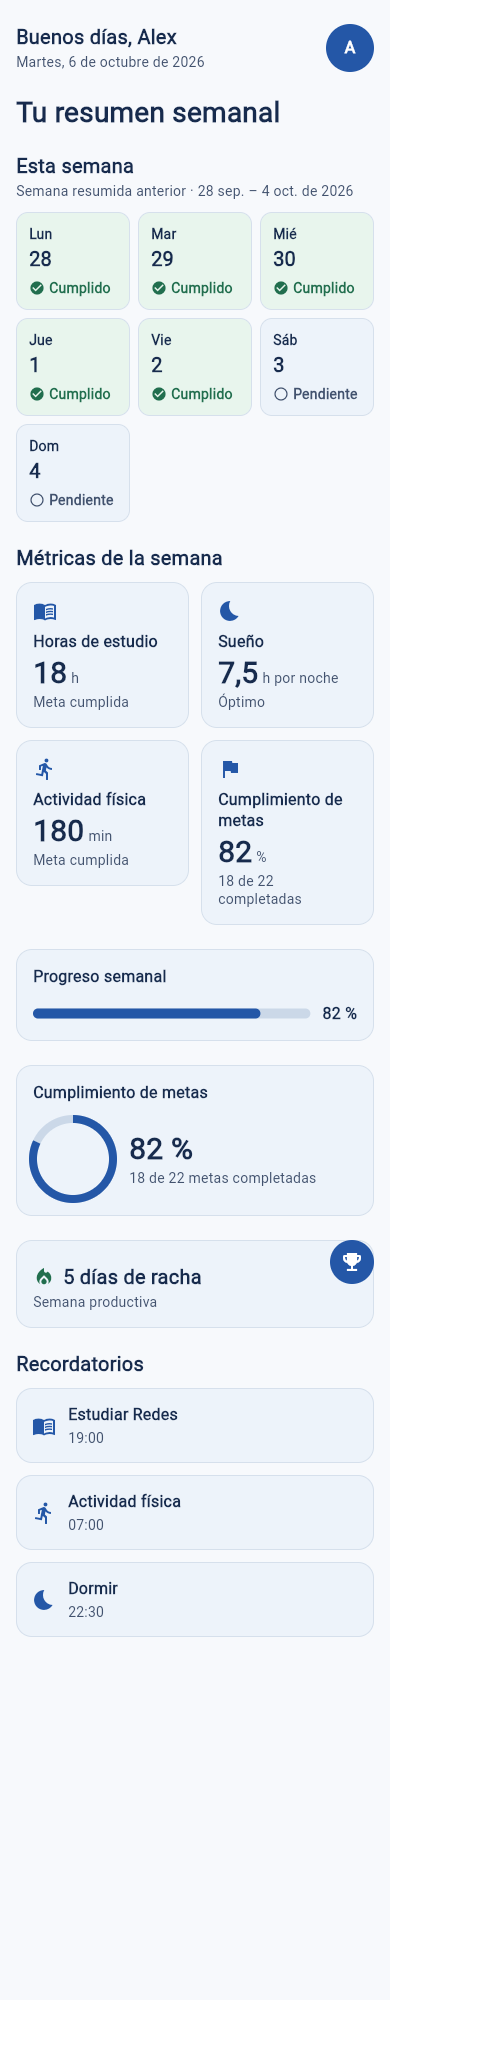
\includegraphics[height=0.73\textheight,keepaspectratio]{vista_movil.png}}{\fbox{\parbox{0.8\textwidth}{Evidencia disponible en build/shots/mobile\_iframe\_390.png. Copiar como vista\_movil.png junto al documento para incluir la imagen.}}}
\caption{Vista móvil preexistente: calendario envuelto, métricas en dos columnas y lectura vertical.}
\end{figure}
\begin{figure}[htbp]
\centering
\IfFileExists{vista_escritorio.png}{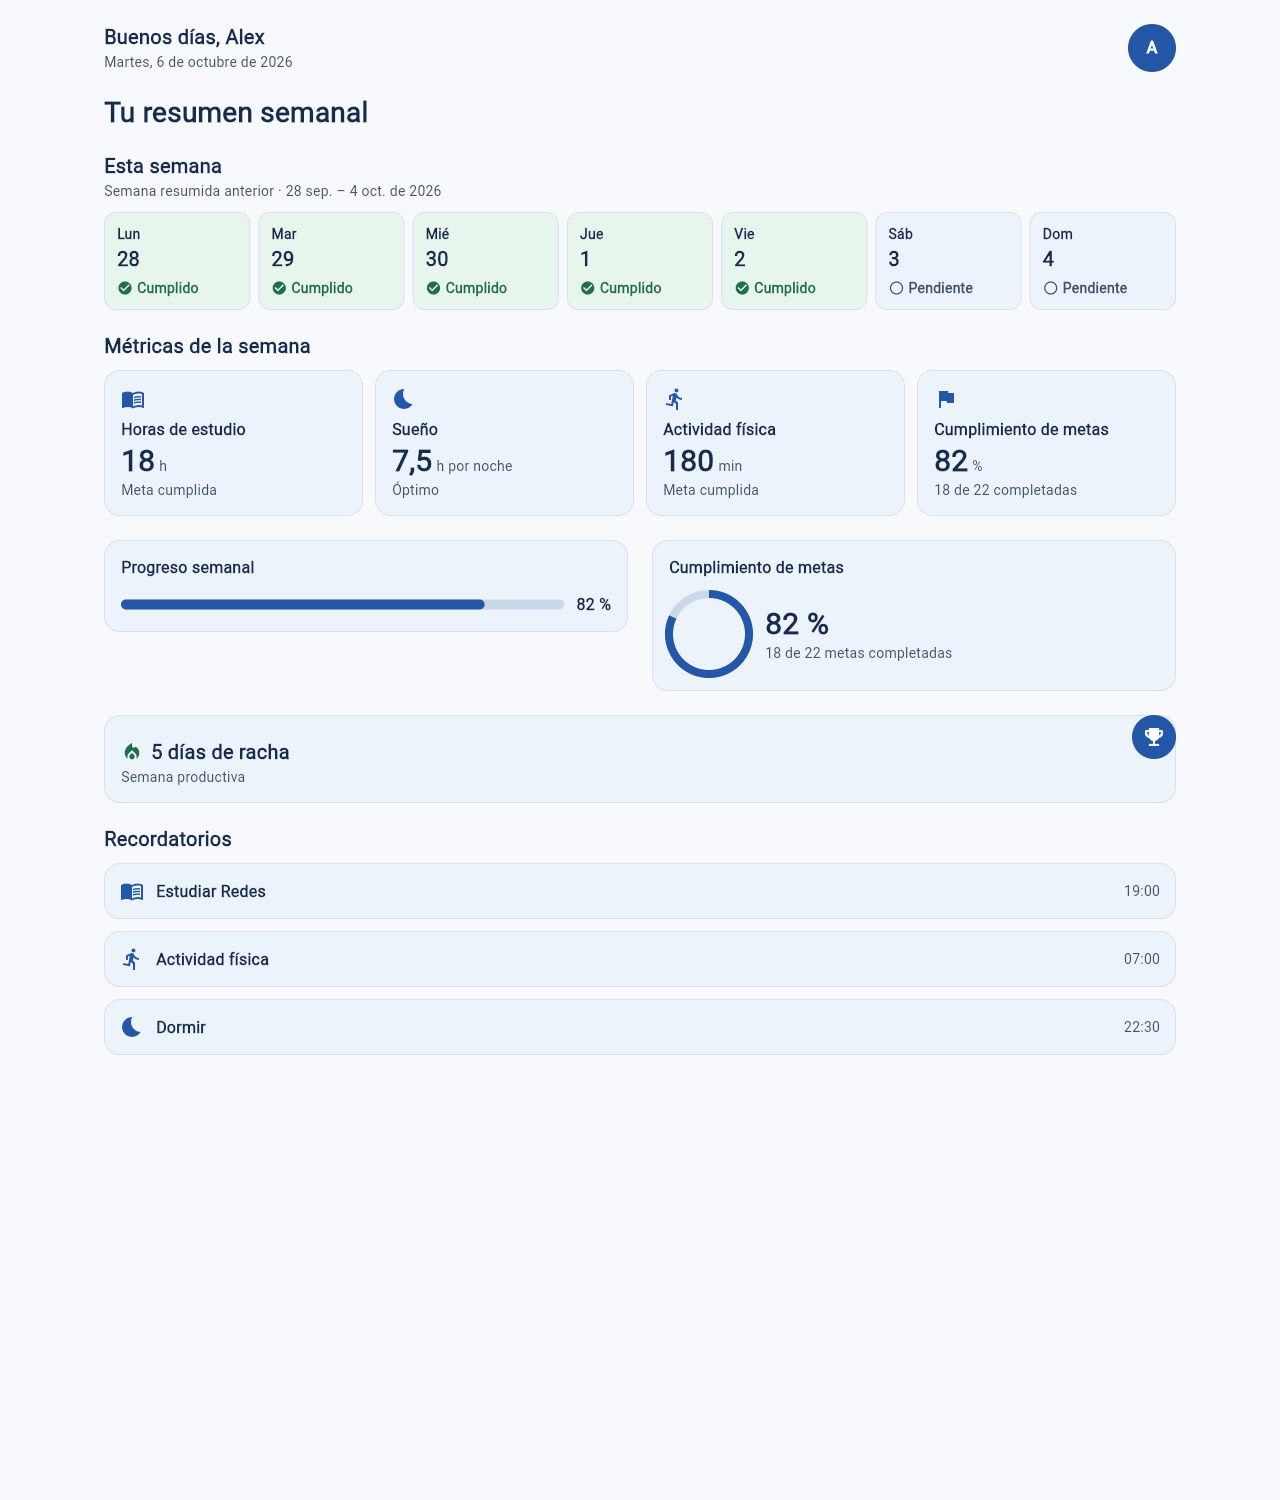
\includegraphics[width=0.92\textwidth,height=0.73\textheight,keepaspectratio]{vista_escritorio.png}}{\fbox{\parbox{0.8\textwidth}{Evidencia disponible en build/shots/wide\_1280.png. Copiar como vista\_escritorio.png junto al documento para incluir la imagen.}}}
\caption{Vista amplia preexistente de 1280 px de ancho: calendario y métricas con distribución horizontal.}
\end{figure}
\clearpage
No se incluye captura de panel de diagnóstico porque no existe ese panel en el código inspeccionado. Las pruebas automatizadas expresan los escenarios de validación previstos, pero no reemplazan la captura de Inspector ni una evaluación manual con tecnologías de asistencia.
\subsection{Análisis de Fragilidad}
La sección de métricas es especialmente sensible al ancho porque combina cuatro contenidos de longitud diferente con valores y unidades. En móvil, la tarjeta de cumplimiento necesita más líneas que las otras; no se fuerza una altura uniforme que pudiera recortar ese contenido. El cambio a una columna con texto grande reduce el riesgo de saturación horizontal.

El calendario también es sensible: siete celdas y la palabra ``Pendiente'' requieren espacio mínimo para conservar legibilidad. El cambio a Wrap distribuye las celdas en varias filas, aumentando la altura total. Los recordatorios resuelven otra fragilidad: nombre y hora compiten por el ancho y por ello la hora se apila en condiciones estrechas. Las pruebas existentes no cubren todas las combinaciones de texto, anchura y escalado; aún es pertinente revisar los límites exactos de cada breakpoint.
\section{Dificultades Encontradas y Soluciones}
La documentación y el código explican medidas preventivas, pero no aportan un historial verificable de errores ocurridos durante el desarrollo. Por ello se describen retos técnicos identificables y soluciones implementadas, sin inventar incidentes ni experiencias personales.
\begin{longtable}{p{4.2cm}p{9.3cm}}
\textbf{Reto identificado} & \textbf{Solución presente}\\\hline
Siete días en ancho reducido & LayoutBuilder alterna Row y Wrap; celdas con ancho finito y estado que puede envolver.\\
Texto y avatar en cabecera & Expanded limita el bloque textual y reserva el avatar de 48 dp.\\
Valor y unidad de métrica & Flexible permite ajustar la unidad; tarjeta sin altura fija.\\
Dos indicadores en móvil & Column sustituye a Row; porcentaje circular fuera de la caja de 80 dp.\\
Trofeo sobre el logro & Positioned junto con padding superior y lateral reservado.\\
Nombre y hora del recordatorio & Hora debajo del nombre si ancho local menor de 360 dp o texto grande.\\
Lista dentro del scroll & shrinkWrap y desplazamiento interno deshabilitado; un único scroll de página.\\\hline
\end{longtable}
Como aprendizaje técnico derivado de la solución, adaptar una interfaz exige distinguir las restricciones del padre del tamaño global de la ventana. El uso correcto de flexibles depende de que su eje tenga límites finitos. También se observa que conservar el escalado tipográfico requiere cambiar la distribución, no reducir artificialmente el texto. Estas conclusiones se basan en la implementación y no se atribuyen como testimonios personales a integrantes no identificados.
\section{Conclusiones}
La implementación cumple el alcance de una pantalla estática con widgets propios sin estado, datos mock y componentes reutilizables. La jerarquía visual organiza calendario, métricas, progreso, logro y recordatorios, y las reglas locales permiten reorganizar el contenido según ancho y tamaño de texto.

La composición de widgets y el modelo de restricciones son centrales: filas flexibles requieren ancho acotado, las cajas de indicadores requieren dimensiones finitas y el contenido vertical necesita una estrategia de desplazamiento coherente. La centralización de estilos facilita mantener consistencia y la semántica añadida mejora la descripción de elementos importantes.

La evidencia disponible respalda la composición visual en las capturas seleccionadas y la existencia de escenarios de prueba. Permanecen pendientes la confirmación de resultados de análisis y pruebas, la evidencia de Inspector, la auditoría de contraste y una revisión con lector de pantalla. Por tanto, el informe no declara una validación exhaustiva ni una puntuación oficial.

Como mejoras futuras se propone completar esas verificaciones, revisar anchos en torno a los breakpoints y ampliar pruebas con textos largos. En una unidad posterior podría incorporarse estado para registrar hábitos, calcular métricas reales y activar recordatorios, manteniendo esas funciones fuera de esta entrega.
\section{Anexos}
\subsection*{Anexo A: Código fuente completo de la aplicación y pruebas}
\addcontentsline{toc}{subsection}{Anexo A: Código fuente completo de la aplicación y pruebas}
Se reproduce el código completo de \codigo{lib}, la suite de \codigo{test} y la configuración principal. Los archivos generados de Android, web, build y herramientas no se transcriben porque no contienen la composición propia de la UI. La copia corresponde a los archivos inspeccionados en \codigo{E:\desII}. No se identificó una URL de repositorio que permita sustituir este anexo por un enlace.
\subsubsection*{\codigo{lib/main.dart}}
\begin{lstlisting}
import 'package:flutter/material.dart';

import 'screens/weekly_summary_screen.dart';
import 'utils/app_constants.dart';

void main() {
  runApp(const ResumenSemanalApp());
}

/// Aplicación de una sola pantalla con tema Material 3.
class ResumenSemanalApp extends StatelessWidget {
  const ResumenSemanalApp({super.key});

  @override
  Widget build(BuildContext context) {
    return MaterialApp(
      title: 'Resumen semanal',
      debugShowCheckedModeBanner: false,
      theme: ThemeData(
        useMaterial3: true,
        colorScheme: ColorScheme.fromSeed(
          seedColor: AppColors.accent,
          brightness: Brightness.light,
        ),
        scaffoldBackgroundColor: AppColors.background,
      ),
      home: const WeeklySummaryScreen(),
    );
  }
}

\end{lstlisting}

\subsubsection*{\codigo{lib/screens/weekly_summary_screen.dart}}
\begin{lstlisting}
import 'package:flutter/material.dart';

import '../utils/app_constants.dart';
import '../widgets/achievement_card.dart';
import '../widgets/header_section.dart';
import '../widgets/metric_card.dart';
import '../widgets/progress_summary.dart';
import '../widgets/reminder_card.dart';
import '../widgets/weekly_calendar.dart';

/// Pantalla única «Resumen semanal de hábitos de estudio y bienestar».
class WeeklySummaryScreen extends StatelessWidget {
  const WeeklySummaryScreen({super.key});

  /// Ancho máximo del contenido, centrado en viewports amplios.
  static const double _maxContentWidth = 1120;

  /// Por debajo de este ancho de viewport se usa un padding más compacto.
  static const double _compactViewportWidth = 600;

  @override
  Widget build(BuildContext context) {
    final MediaQueryData mediaQuery = MediaQuery.of(context);
    final double horizontalPadding =
        mediaQuery.size.width < _compactViewportWidth ? 16 : 24;

    return Scaffold(
      backgroundColor: AppColors.background,
      body: SafeArea(
        child: SingleChildScrollView(
          child: Center(
            child: ConstrainedBox(
              constraints: const BoxConstraints(maxWidth: _maxContentWidth),
              child: Padding(
                padding: EdgeInsets.symmetric(
                  horizontal: horizontalPadding,
                  vertical: AppSpacing.xl,
                ),
                child: LayoutBuilder(
                  builder: (BuildContext context, BoxConstraints constraints) {
                    // Column bajo scroll: sin flexibles verticales.
                    return Column(
                      mainAxisSize: MainAxisSize.min,
                      crossAxisAlignment: CrossAxisAlignment.stretch,
                      children: <Widget>[
                        const HeaderSection(),
                        const SizedBox(height: AppSpacing.sectionSpacing),
                        const Text(
                          MockData.screenTitle,
                          style: AppTextStyles.screenTitle,
                        ),
                        const SizedBox(height: AppSpacing.sectionSpacing),
                        const WeeklyCalendar(),
                        const SizedBox(height: AppSpacing.sectionSpacing),
                        const _MetricsSection(),
                        const SizedBox(height: AppSpacing.sectionSpacing),
                        const ProgressSummary(),
                        const SizedBox(height: AppSpacing.sectionSpacing),
                        const AchievementCard(),
                        const SizedBox(height: AppSpacing.sectionSpacing),
                        const _RemindersSection(),
                      ],
                    );
                  },
                ),
              ),
            ),
          ),
        ),
      ),
    );
  }
}

/// Métricas en Wrap: cuatro columnas si hay ancho y texto normal, dos columnas
/// por debajo y una columna como salvaguarda para texto grande o ancho mínimo.
class _MetricsSection extends StatelessWidget {
  const _MetricsSection();

  static const double _fourColumnMinWidth = 900;
  static const double _singleColumnMaxWidth = 280;

  @override
  Widget build(BuildContext context) {
    final bool largeText =
        MediaQuery.textScalerOf(context).scale(AppTypography.body) >
        AppTypography.largeTextThreshold;

    return Column(
      crossAxisAlignment: CrossAxisAlignment.start,
      children: <Widget>[
        const Text(
          MockData.metricsSectionTitle,
          style: AppTextStyles.sectionTitle,
        ),
        const SizedBox(height: AppSpacing.md),
        LayoutBuilder(
          builder: (BuildContext context, BoxConstraints constraints) {
            final double availableWidth = constraints.maxWidth;
            final int columns;
            if (largeText || availableWidth < _singleColumnMaxWidth) {
              columns = 1;
            } else if (availableWidth >= _fourColumnMinWidth) {
              columns = 4;
            } else {
              columns = 2;
            }
            final double cardWidth =
                (availableWidth - AppSpacing.metricSpacing * (columns - 1)) /
                columns;
            return Wrap(
              spacing: AppSpacing.metricSpacing,
              runSpacing: AppSpacing.metricSpacing,
              children: <Widget>[
                for (final WeeklyMetric metric in MockData.metrics)
                  SizedBox(
                    width: cardWidth,
                    child: MetricCard(
                      icon: metric.icon,
                      name: metric.name,
                      value: metric.value,
                      unit: metric.unit,
                      status: metric.status,
                    ),
                  ),
              ],
            );
          },
        ),
      ],
    );
  }
}

/// Recordatorios en una lista corta anidada: el scroll lo hace la página.
class _RemindersSection extends StatelessWidget {
  const _RemindersSection();

  @override
  Widget build(BuildContext context) {
    return Column(
      crossAxisAlignment: CrossAxisAlignment.start,
      children: <Widget>[
        const Text(
          MockData.remindersSectionTitle,
          style: AppTextStyles.sectionTitle,
        ),
        const SizedBox(height: AppSpacing.md),
        ListView.separated(
          shrinkWrap: true,
          primary: false,
          physics: const NeverScrollableScrollPhysics(),
          itemCount: MockData.reminders.length,
          separatorBuilder: (BuildContext context, int index) =>
              const SizedBox(height: AppSpacing.md),
          itemBuilder: (BuildContext context, int index) {
            final StudyReminder reminder = MockData.reminders[index];
            return ReminderCard(
              icon: reminder.icon,
              name: reminder.name,
              time: reminder.time,
            );
          },
        ),
      ],
    );
  }
}

\end{lstlisting}

\subsubsection*{\codigo{lib/utils/app_constants.dart}}
\begin{lstlisting}
import 'package:flutter/material.dart';

/// Colores y superficies de la dirección visual (inspiración conceptual en
/// Google Fit: calma, espacio en blanco y tarjetas suaves).
abstract final class AppColors {
  static const Color background = Color(0xFFF7F9FC);
  static const Color surface = Color(0xFFFFFFFF);
  static const Color softCard = Color(0xFFEDF3FA);
  static const Color textPrimary = Color(0xFF172B4D);
  static const Color textSecondary = Color(0xFF42526E);
  static const Color accent = Color(0xFF2457A7);
  static const Color success = Color(0xFF216E4E);
  static const Color successSurface = Color(0xFFE8F5ED);
  static const Color subtleBorder = Color(0xFFD6E0EC);
  static const Color track = Color(0xFFCBD8E8);
}

/// Escala de separación: 4, 8, 12, 16, 24 y 32 dp.
abstract final class AppSpacing {
  static const double xs = 4;
  static const double sm = 8;
  static const double md = 12;
  static const double lg = 16;
  static const double xl = 24;
  static const double xxl = 32;

  static const double cardPadding = 16;
  static const double metricSpacing = 12;
  static const double sectionSpacing = 24;
}

/// Radios consistentes: tarjetas 16, chips 12, indicadores 8.
abstract final class AppRadii {
  static const double card = 16;
  static const double chip = 12;
  static const double indicator = 8;
}

/// Tamaños de la jerarquía tipográfica en sp.
abstract final class AppTypography {
  static const double screenTitle = 28;
  static const double sectionTitle = 20;
  static const double metricValue = 30;
  static const double body = 16;
  static const double secondary = 14;

  /// Umbral para considerar «texto grande»: scale(16) > 20.
  static const double largeTextThreshold = 20;
}

/// Estilos de texto derivados de la jerarquía tipográfica.
abstract final class AppTextStyles {
  static const TextStyle screenTitle = TextStyle(
    fontSize: AppTypography.screenTitle,
    fontWeight: FontWeight.w700,
    color: AppColors.textPrimary,
    height: 1.2,
  );

  static const TextStyle sectionTitle = TextStyle(
    fontSize: AppTypography.sectionTitle,
    fontWeight: FontWeight.w600,
    color: AppColors.textPrimary,
    height: 1.2,
  );

  static const TextStyle metricValue = TextStyle(
    fontSize: AppTypography.metricValue,
    fontWeight: FontWeight.w700,
    color: AppColors.textPrimary,
    height: 1.1,
  );

  static const TextStyle body = TextStyle(
    fontSize: AppTypography.body,
    color: AppColors.textPrimary,
    height: 1.3,
  );

  static const TextStyle bodyStrong = TextStyle(
    fontSize: AppTypography.body,
    fontWeight: FontWeight.w600,
    color: AppColors.textPrimary,
    height: 1.3,
  );

  static const TextStyle secondary = TextStyle(
    fontSize: AppTypography.secondary,
    color: AppColors.textSecondary,
    height: 1.3,
  );

  static const TextStyle secondaryStrong = TextStyle(
    fontSize: AppTypography.secondary,
    fontWeight: FontWeight.w600,
    color: AppColors.textPrimary,
    height: 1.3,
  );
}

/// Estado de un día de la semana resumida.
enum DayStatus {
  completed('Cumplido'),
  pending('Pendiente');

  const DayStatus(this.label);

  /// Etiqueta textual que acompaña al icono: el estado nunca depende del color.
  final String label;
}

/// Día del calendario semanal (dato mock inmutable).
@immutable
class StudyDay {
  const StudyDay({
    required this.abbreviation,
    required this.dayNumber,
    required this.status,
  });

  final String abbreviation;
  final int dayNumber;
  final DayStatus status;
}

/// Métrica semanal (dato mock inmutable).
@immutable
class WeeklyMetric {
  const WeeklyMetric({
    required this.icon,
    required this.name,
    required this.value,
    required this.unit,
    required this.status,
  });

  final IconData icon;
  final String name;
  final String value;
  final String unit;
  final String status;
}

/// Recordatorio de ejemplo (dato mock inmutable, sin acciones).
@immutable
class StudyReminder {
  const StudyReminder({
    required this.icon,
    required this.name,
    required this.time,
  });

  final IconData icon;
  final String name;
  final String time;
}

/// Datos constantes de la pantalla. No se calcula ninguna métrica de negocio;
/// los porcentajes son valores mock suministrados.
abstract final class MockData {
  static const String greeting = 'Buenos días, Alex';
  static const String todayLabel = 'Martes, 6 de octubre de 2026';
  static const String avatarInitial = 'A';
  static const String avatarSemantics = 'Perfil de ejemplo';
  static const String screenTitle = 'Tu resumen semanal';
  static const String weekSectionTitle = 'Esta semana';
  static const String weekRangeLabel =
      'Semana resumida anterior · 28 sep. – 4 oct. de 2026';
  static const String metricsSectionTitle = 'Métricas de la semana';
  static const String remindersSectionTitle = 'Recordatorios';
  static const String achievementTitle = '5 días de racha';
  static const String achievementSubtitle = 'Semana productiva';
  static const String achievementBadgeSemantics = 'Insignia de trofeo';

  // Progreso semanal y cumplimiento: valores constantes suministrados.
  static const String weeklyProgressTitle = 'Progreso semanal';
  static const String weeklyProgressLabel = '82 %';
  static const double weeklyProgressValue = 0.82;

  static const String goalsProgressTitle = 'Cumplimiento de metas';
  static const String goalsProgressLabel = '82 %';
  static const String goalsProgressCaption = '18 de 22 metas completadas';
  static const double goalsProgressValue = 0.82;

  static const List<StudyDay> weekDays = <StudyDay>[
    StudyDay(abbreviation: 'Lun', dayNumber: 28, status: DayStatus.completed),
    StudyDay(abbreviation: 'Mar', dayNumber: 29, status: DayStatus.completed),
    StudyDay(abbreviation: 'Mié', dayNumber: 30, status: DayStatus.completed),
    StudyDay(abbreviation: 'Jue', dayNumber: 1, status: DayStatus.completed),
    StudyDay(abbreviation: 'Vie', dayNumber: 2, status: DayStatus.completed),
    StudyDay(abbreviation: 'Sáb', dayNumber: 3, status: DayStatus.pending),
    StudyDay(abbreviation: 'Dom', dayNumber: 4, status: DayStatus.pending),
  ];

  static const List<WeeklyMetric> metrics = <WeeklyMetric>[
    WeeklyMetric(
      icon: Icons.menu_book,
      name: 'Horas de estudio',
      value: '18',
      unit: 'h',
      status: 'Meta cumplida',
    ),
    WeeklyMetric(
      icon: Icons.bedtime,
      name: 'Sueño',
      value: '7,5',
      unit: 'h por noche',
      status: 'Óptimo',
    ),
    WeeklyMetric(
      icon: Icons.directions_run,
      name: 'Actividad física',
      value: '180',
      unit: 'min',
      status: 'Meta cumplida',
    ),
    WeeklyMetric(
      icon: Icons.flag,
      name: 'Cumplimiento de metas',
      value: '82',
      unit: '%',
      status: '18 de 22 completadas',
    ),
  ];

  static const List<StudyReminder> reminders = <StudyReminder>[
    StudyReminder(icon: Icons.menu_book, name: 'Estudiar Redes', time: '19:00'),
    StudyReminder(
      icon: Icons.directions_run,
      name: 'Actividad física',
      time: '07:00',
    ),
    StudyReminder(icon: Icons.bedtime, name: 'Dormir', time: '22:30'),
  ];
}

\end{lstlisting}

\subsubsection*{\codigo{lib/widgets/header_section.dart}}
\begin{lstlisting}
import 'package:flutter/material.dart';

import '../utils/app_constants.dart';

/// Encabezado con saludo, fecha fija y avatar de ejemplo. Sin interacción.
class HeaderSection extends StatelessWidget {
  const HeaderSection({super.key});

  @override
  Widget build(BuildContext context) {
    return Row(
      children: <Widget>[
        Expanded(
          child: Column(
            crossAxisAlignment: CrossAxisAlignment.start,
            children: const <Widget>[
              Text(MockData.greeting, style: AppTextStyles.sectionTitle),
              SizedBox(height: AppSpacing.xs),
              Text(MockData.todayLabel, style: AppTextStyles.secondary),
            ],
          ),
        ),
        const SizedBox(width: AppSpacing.lg),
        // El avatar describe un perfil de ejemplo; no anuncia ninguna acción.
        Semantics(
          container: true,
          excludeSemantics: true,
          label: MockData.avatarSemantics,
          child: const CircleAvatar(
            radius: 24,
            backgroundColor: AppColors.accent,
            child: Text(
              MockData.avatarInitial,
              style: TextStyle(
                fontSize: AppTypography.body,
                fontWeight: FontWeight.w600,
                color: AppColors.surface,
              ),
            ),
          ),
        ),
      ],
    );
  }
}

\end{lstlisting}

\subsubsection*{\codigo{lib/widgets/weekly_calendar.dart}}
\begin{lstlisting}
import 'package:flutter/material.dart';

import '../utils/app_constants.dart';

/// Calendario de la semana resumida con los siete días y su estado.
class WeeklyCalendar extends StatelessWidget {
  const WeeklyCalendar({super.key});

  /// Desde este ancho local se usa una fila con siete celdas expandidas.
  static const double _rowMinWidth = 700;

  /// Ancho mínimo aproximado por celda en el diseño envuelto (Wrap).
  static const double _wrapCellMinWidth = 96;

  /// Ancho mínimo por celda cuando el texto del sistema está ampliado.
  static const double _wrapCellMinWidthLargeText = 128;

  static const double _wrapSpacing = 8;
  static const int _maxColumns = 7;

  @override
  Widget build(BuildContext context) {
    final bool largeText =
        MediaQuery.textScalerOf(context).scale(AppTypography.body) >
        AppTypography.largeTextThreshold;

    return Column(
      crossAxisAlignment: CrossAxisAlignment.start,
      children: <Widget>[
        const Text(
          MockData.weekSectionTitle,
          style: AppTextStyles.sectionTitle,
        ),
        const SizedBox(height: AppSpacing.xs),
        const Text(MockData.weekRangeLabel, style: AppTextStyles.secondary),
        const SizedBox(height: AppSpacing.md),
        LayoutBuilder(
          builder: (BuildContext context, BoxConstraints constraints) {
            final double availableWidth = constraints.maxWidth;
            if (!largeText && availableWidth >= _rowMinWidth) {
              return _buildRowCalendar();
            }
            return _buildWrappedCalendar(availableWidth, largeText);
          },
        ),
      ],
    );
  }

  /// Fila con siete celdas expandidas para anchos amplios y texto normal.
  Widget _buildRowCalendar() {
    final int lastIndex = MockData.weekDays.length - 1;
    return Row(
      crossAxisAlignment: CrossAxisAlignment.start,
      children: <Widget>[
        for (int i = 0; i <= lastIndex; i++) ...<Widget>[
          Expanded(child: _DayCell(day: MockData.weekDays[i])),
          if (i != lastIndex) const SizedBox(width: _wrapSpacing),
        ],
      ],
    );
  }

  /// Envoltura con celdas de ancho finito para anchos estrechos o texto grande.
  /// Nunca se coloca Expanded dentro de un Wrap.
  Widget _buildWrappedCalendar(double availableWidth, bool largeText) {
    final double minCellWidth = largeText
        ? _wrapCellMinWidthLargeText
        : _wrapCellMinWidth;
    final int columns =
        ((availableWidth + _wrapSpacing) / (minCellWidth + _wrapSpacing))
            .floor()
            .clamp(1, _maxColumns);
    final double cellWidth =
        (availableWidth - _wrapSpacing * (columns - 1)) / columns;
    return Wrap(
      spacing: _wrapSpacing,
      runSpacing: _wrapSpacing,
      children: <Widget>[
        for (final StudyDay day in MockData.weekDays)
          SizedBox(
            width: cellWidth,
            child: _DayCell(day: day),
          ),
      ],
    );
  }
}

/// Celda de un día: abreviatura, número y estado con icono y texto.
class _DayCell extends StatelessWidget {
  const _DayCell({required this.day});

  final StudyDay day;

  @override
  Widget build(BuildContext context) {
    final bool completed = day.status == DayStatus.completed;
    final Color statusColor = completed
        ? AppColors.success
        : AppColors.textSecondary;
    final Color surfaceColor = completed
        ? AppColors.successSurface
        : AppColors.softCard;
    final IconData statusIcon = completed
        ? Icons.check_circle
        : Icons.radio_button_unchecked;

    // El estado no depende del color: icono + texto lo describen.
    return Semantics(
      container: true,
      excludeSemantics: true,
      label: '${day.abbreviation} ${day.dayNumber}, ${day.status.label}',
      child: Container(
        padding: const EdgeInsets.all(AppSpacing.md),
        decoration: BoxDecoration(
          color: surfaceColor,
          borderRadius: BorderRadius.circular(AppRadii.chip),
          border: Border.all(color: AppColors.subtleBorder),
        ),
        child: Column(
          crossAxisAlignment: CrossAxisAlignment.start,
          children: <Widget>[
            Text(day.abbreviation, style: AppTextStyles.secondaryStrong),
            const SizedBox(height: AppSpacing.xs),
            Text('${day.dayNumber}', style: AppTextStyles.sectionTitle),
            const SizedBox(height: AppSpacing.sm),
            // Wrap evita que el estado se recorte en celdas estrechas: el
            // icono y el texto pasan a renglones distintos si hace falta.
            Wrap(
              spacing: AppSpacing.xs,
              runSpacing: AppSpacing.xs,
              crossAxisAlignment: WrapCrossAlignment.center,
              children: <Widget>[
                Icon(statusIcon, size: 16, color: statusColor),
                Text(
                  day.status.label,
                  style: TextStyle(
                    fontSize: AppTypography.secondary,
                    fontWeight: FontWeight.w600,
                    color: statusColor,
                    height: 1.3,
                  ),
                ),
              ],
            ),
          ],
        ),
      ),
    );
  }
}

\end{lstlisting}

\subsubsection*{\codigo{lib/widgets/metric_card.dart}}
\begin{lstlisting}
import 'package:flutter/material.dart';

import '../utils/app_constants.dart';

/// Tarjeta de una métrica semanal: icono, nombre, valor, unidad y estado.
/// Sin altura fija: la tarjeta crece según su contenido.
class MetricCard extends StatelessWidget {
  const MetricCard({
    super.key,
    required this.icon,
    required this.name,
    required this.value,
    required this.unit,
    required this.status,
  });

  final IconData icon;
  final String name;
  final String value;
  final String unit;
  final String status;

  @override
  Widget build(BuildContext context) {
    return Container(
      padding: const EdgeInsets.all(AppSpacing.cardPadding),
      decoration: BoxDecoration(
        color: AppColors.softCard,
        borderRadius: BorderRadius.circular(AppRadii.card),
        border: Border.all(color: AppColors.subtleBorder),
      ),
      child: Column(
        crossAxisAlignment: CrossAxisAlignment.start,
        children: <Widget>[
          Icon(icon, size: 24, color: AppColors.accent),
          const SizedBox(height: AppSpacing.sm),
          Text(name, style: AppTextStyles.bodyStrong),
          const SizedBox(height: AppSpacing.xs),
          Row(
            crossAxisAlignment: CrossAxisAlignment.baseline,
            textBaseline: TextBaseline.alphabetic,
            children: <Widget>[
              Text(value, style: AppTextStyles.metricValue),
              const SizedBox(width: AppSpacing.xs),
              Flexible(child: Text(unit, style: AppTextStyles.secondary)),
            ],
          ),
          const SizedBox(height: AppSpacing.xs),
          Text(status, style: AppTextStyles.secondary),
        ],
      ),
    );
  }
}

\end{lstlisting}

\subsubsection*{\codigo{lib/widgets/progress_summary.dart}}
\begin{lstlisting}
import 'package:flutter/material.dart';

import '../utils/app_constants.dart';

/// Resumen de progreso: barra semanal lineal y cumplimiento circular, ambos
/// con valor determinado y porcentaje visible.
class ProgressSummary extends StatelessWidget {
  const ProgressSummary({super.key});

  /// Desde este ancho local ambos bloques comparten una fila (si el texto es
  /// normal); en otro caso se apilan en columna.
  static const double _rowMinWidth = 600;

  @override
  Widget build(BuildContext context) {
    final bool largeText =
        MediaQuery.textScalerOf(context).scale(AppTypography.body) >
        AppTypography.largeTextThreshold;

    return LayoutBuilder(
      builder: (BuildContext context, BoxConstraints constraints) {
        const Widget weekly = _LinearProgressBlock();
        const Widget goals = _CircularProgressBlock();

        if (!largeText && constraints.maxWidth >= _rowMinWidth) {
          return Row(
            crossAxisAlignment: CrossAxisAlignment.start,
            children: const <Widget>[
              Expanded(child: weekly),
              SizedBox(width: AppSpacing.xl),
              Expanded(child: goals),
            ],
          );
        }
        return const Column(
          crossAxisAlignment: CrossAxisAlignment.stretch,
          children: <Widget>[
            weekly,
            SizedBox(height: AppSpacing.xl),
            goals,
          ],
        );
      },
    );
  }
}

/// Progreso semanal con LinearProgressIndicator determinado.
class _LinearProgressBlock extends StatelessWidget {
  const _LinearProgressBlock();

  @override
  Widget build(BuildContext context) {
    return const _ProgressCard(
      title: MockData.weeklyProgressTitle,
      semanticsLabel: MockData.weeklyProgressTitle,
      semanticsValue: MockData.weeklyProgressLabel,
      child: Row(
        children: <Widget>[
          Expanded(
            child: LinearProgressIndicator(
              value: MockData.weeklyProgressValue,
              minHeight: 10,
              borderRadius: BorderRadius.all(
                Radius.circular(AppRadii.indicator),
              ),
              backgroundColor: AppColors.track,
              color: AppColors.accent,
            ),
          ),
          SizedBox(width: AppSpacing.md),
          Text(MockData.weeklyProgressLabel, style: AppTextStyles.bodyStrong),
        ],
      ),
    );
  }
}

/// Cumplimiento de metas con CircularProgressIndicator determinado.
class _CircularProgressBlock extends StatelessWidget {
  const _CircularProgressBlock();

  @override
  Widget build(BuildContext context) {
    return const _ProgressCard(
      title: MockData.goalsProgressTitle,
      semanticsLabel: MockData.goalsProgressTitle,
      semanticsValue: MockData.goalsProgressLabel,
      child: Row(
        crossAxisAlignment: CrossAxisAlignment.center,
        children: <Widget>[
          // El indicador vive en un SizedBox finito de 80 x 80.
          SizedBox(
            width: 80,
            height: 80,
            child: CircularProgressIndicator(
              value: MockData.goalsProgressValue,
              strokeWidth: 8,
              backgroundColor: AppColors.track,
              color: AppColors.accent,
            ),
          ),
          SizedBox(width: AppSpacing.lg),
          // El porcentaje va fuera del círculo para admitir escalado sin cortes.
          Expanded(
            child: Column(
              crossAxisAlignment: CrossAxisAlignment.start,
              mainAxisSize: MainAxisSize.min,
              children: <Widget>[
                Text(
                  MockData.goalsProgressLabel,
                  style: AppTextStyles.metricValue,
                ),
                SizedBox(height: AppSpacing.xs),
                Text(
                  MockData.goalsProgressCaption,
                  style: AppTextStyles.secondary,
                ),
              ],
            ),
          ),
        ],
      ),
    );
  }
}

/// Tarjeta común de un bloque de progreso con descripción accesible propia.
class _ProgressCard extends StatelessWidget {
  const _ProgressCard({
    required this.title,
    required this.semanticsLabel,
    required this.semanticsValue,
    required this.child,
  });

  final String title;
  final String semanticsLabel;
  final String semanticsValue;
  final Widget child;

  @override
  Widget build(BuildContext context) {
    // excludeSemantics evita que el lector repita el texto visible.
    return Semantics(
      container: true,
      excludeSemantics: true,
      label: semanticsLabel,
      value: semanticsValue,
      child: Container(
        padding: const EdgeInsets.all(AppSpacing.cardPadding),
        decoration: BoxDecoration(
          color: AppColors.softCard,
          borderRadius: BorderRadius.circular(AppRadii.card),
          border: Border.all(color: AppColors.subtleBorder),
        ),
        child: Column(
          crossAxisAlignment: CrossAxisAlignment.start,
          children: <Widget>[
            Text(title, style: AppTextStyles.bodyStrong),
            const SizedBox(height: AppSpacing.lg),
            child,
          ],
        ),
      ),
    );
  }
}

\end{lstlisting}

\subsubsection*{\codigo{lib/widgets/achievement_card.dart}}
\begin{lstlisting}
import 'package:flutter/material.dart';

import '../utils/app_constants.dart';

/// Tarjeta de logro con insignia de trofeo superpuesta en la esquina superior.
class AchievementCard extends StatelessWidget {
  const AchievementCard({super.key});

  /// Espacio reservado arriba para que la insignia no tape el texto.
  static const double _topReservedSpace = 24;

  /// Espacio reservado a la derecha para que la insignia no tape el texto.
  static const double _sideReservedSpace = 56;

  @override
  Widget build(BuildContext context) {
    return Stack(
      children: <Widget>[
        Container(
          width: double.infinity,
          padding: const EdgeInsets.fromLTRB(
            AppSpacing.cardPadding,
            _topReservedSpace,
            _sideReservedSpace,
            AppSpacing.cardPadding,
          ),
          decoration: BoxDecoration(
            color: AppColors.softCard,
            borderRadius: BorderRadius.circular(AppRadii.card),
            border: Border.all(color: AppColors.subtleBorder),
          ),
          child: Column(
            crossAxisAlignment: CrossAxisAlignment.start,
            children: <Widget>[
              Row(
                children: <Widget>[
                  const Icon(
                    Icons.local_fire_department,
                    size: 22,
                    color: AppColors.success,
                  ),
                  const SizedBox(width: AppSpacing.sm),
                  Expanded(
                    child: Text(
                      MockData.achievementTitle,
                      style: AppTextStyles.sectionTitle,
                    ),
                  ),
                ],
              ),
              const SizedBox(height: AppSpacing.xs),
              Text(
                MockData.achievementSubtitle,
                style: AppTextStyles.secondary,
              ),
            ],
          ),
        ),
        const Positioned(top: 0, right: 0, child: _AchievementBadge()),
      ],
    );
  }
}

/// Insignia de trofeo dentro de los límites del Stack.
class _AchievementBadge extends StatelessWidget {
  const _AchievementBadge();

  @override
  Widget build(BuildContext context) {
    return Container(
      width: 44,
      height: 44,
      decoration: const BoxDecoration(
        color: AppColors.accent,
        shape: BoxShape.circle,
      ),
      child: const Icon(
        Icons.emoji_events,
        size: 24,
        color: AppColors.surface,
        semanticLabel: MockData.achievementBadgeSemantics,
      ),
    );
  }
}

\end{lstlisting}

\subsubsection*{\codigo{lib/widgets/reminder_card.dart}}
\begin{lstlisting}
import 'package:flutter/material.dart';

import '../utils/app_constants.dart';

/// Recordatorio de ejemplo: icono, nombre y hora. Sin acciones funcionales.
class ReminderCard extends StatelessWidget {
  const ReminderCard({
    super.key,
    required this.icon,
    required this.name,
    required this.time,
  });

  final IconData icon;
  final String name;
  final String time;

  /// Por debajo de este ancho local (o con texto grande) la hora baja al
  /// segundo renglón para evitar desbordes.
  static const double _stackMaxWidth = 360;

  @override
  Widget build(BuildContext context) {
    final bool largeText =
        MediaQuery.textScalerOf(context).scale(AppTypography.body) >
        AppTypography.largeTextThreshold;

    return LayoutBuilder(
      builder: (BuildContext context, BoxConstraints constraints) {
        final bool stackTime =
            largeText || constraints.maxWidth < _stackMaxWidth;
        final Text nameText = Text(name, style: AppTextStyles.bodyStrong);
        final Text timeText = Text(time, style: AppTextStyles.secondary);

        return Card(
          margin: EdgeInsets.zero,
          elevation: 0,
          color: AppColors.softCard,
          shape: RoundedRectangleBorder(
            borderRadius: BorderRadius.circular(AppRadii.card),
            side: const BorderSide(color: AppColors.subtleBorder),
          ),
          child: Padding(
            padding: const EdgeInsets.all(AppSpacing.cardPadding),
            child: Row(
              crossAxisAlignment: CrossAxisAlignment.center,
              children: <Widget>[
                Icon(icon, size: 24, color: AppColors.accent),
                const SizedBox(width: AppSpacing.md),
                Expanded(
                  child: stackTime
                      ? Column(
                          crossAxisAlignment: CrossAxisAlignment.start,
                          children: <Widget>[
                            nameText,
                            const SizedBox(height: AppSpacing.xs),
                            timeText,
                          ],
                        )
                      : Row(
                          children: <Widget>[
                            Expanded(child: nameText),
                            const SizedBox(width: AppSpacing.md),
                            timeText,
                          ],
                        ),
                ),
              ],
            ),
          ),
        );
      },
    );
  }
}

\end{lstlisting}

\subsubsection*{\codigo{test/weekly_summary_screen_test.dart}}
\begin{lstlisting}
import 'package:flutter/material.dart';
import 'package:flutter_test/flutter_test.dart';
import 'package:resumen_semanal/screens/weekly_summary_screen.dart';
import 'package:resumen_semanal/utils/app_constants.dart';
import 'package:resumen_semanal/widgets/achievement_card.dart';
import 'package:resumen_semanal/widgets/header_section.dart';
import 'package:resumen_semanal/widgets/metric_card.dart';
import 'package:resumen_semanal/widgets/progress_summary.dart';
import 'package:resumen_semanal/widgets/reminder_card.dart';
import 'package:resumen_semanal/widgets/weekly_calendar.dart';

/// Monta la pantalla con un tamaño de vista y una escala de texto concretos.
Future<void> _pumpScreen(
  WidgetTester tester, {
  required Size size,
  double textScale = 1.0,
}) async {
  tester.view.physicalSize = size;
  tester.view.devicePixelRatio = 1.0;
  addTearDown(tester.view.reset);
  addTearDown(tester.view.resetDevicePixelRatio);

  await tester.pumpWidget(
    MaterialApp(
      debugShowCheckedModeBanner: false,
      home: MediaQuery(
        data: MediaQueryData(
          size: size,
          textScaler: TextScaler.linear(textScale),
        ),
        child: const WeeklySummaryScreen(),
      ),
    ),
  );
  await tester.pump();
}

void main() {
  group('composición de la pantalla', () {
    testWidgets('muestra los seis bloques y los textos fijos', (tester) async {
      await _pumpScreen(tester, size: const Size(390, 844));

      expect(find.byType(HeaderSection), findsOneWidget);
      expect(find.byType(WeeklyCalendar), findsOneWidget);
      expect(find.byType(MetricCard), findsNWidgets(4));
      expect(find.byType(ProgressSummary), findsOneWidget);
      expect(find.byType(AchievementCard), findsOneWidget);
      expect(find.byType(ReminderCard), findsNWidgets(3));

      expect(find.text(MockData.screenTitle), findsOneWidget);
      expect(find.text(MockData.greeting), findsOneWidget);
      expect(find.text(MockData.todayLabel), findsOneWidget);
      expect(find.text(MockData.avatarInitial), findsOneWidget);
      expect(find.text(MockData.weekRangeLabel), findsOneWidget);
    });

    testWidgets('calendario: siete días con estado por texto e icono', (
      tester,
    ) async {
      await _pumpScreen(tester, size: const Size(390, 844));

      for (final String abbreviation in <String>[
        'Lun',
        'Mar',
        'Mié',
        'Jue',
        'Vie',
        'Sáb',
        'Dom',
      ]) {
        expect(find.text(abbreviation), findsOneWidget);
      }
      expect(find.text('Cumplido'), findsNWidgets(5));
      expect(find.text('Pendiente'), findsNWidgets(2));
      expect(find.byIcon(Icons.check_circle), findsNWidgets(5));
      expect(find.byIcon(Icons.radio_button_unchecked), findsNWidgets(2));
    });

    testWidgets(
      'métricas: cada tarjeta tiene icono, nombre, valor, unidad y estado',
      (tester) async {
        await _pumpScreen(tester, size: const Size(1280, 900));

        final Finder metricCards = find.byType(MetricCard);
        expect(metricCards, findsNWidgets(4));

        // Se busca dentro de cada tarjeta porque algunos nombres también
        // aparecen en recordatorios o en los bloques de progreso.
        for (int i = 0; i < MockData.metrics.length; i++) {
          final WeeklyMetric metric = MockData.metrics[i];
          final Finder card = metricCards.at(i);
          expect(
            find.descendant(of: card, matching: find.text(metric.name)),
            findsOneWidget,
          );
          expect(
            find.descendant(of: card, matching: find.text(metric.value)),
            findsOneWidget,
          );
          expect(
            find.descendant(of: card, matching: find.text(metric.unit)),
            findsOneWidget,
          );
          expect(
            find.descendant(of: card, matching: find.text(metric.status)),
            findsOneWidget,
          );
          expect(
            find.descendant(of: card, matching: find.byType(Icon)),
            findsOneWidget,
          );
        }
      },
    );
  });

  group('indicadores de progreso', () {
    testWidgets('valores determinados y porcentaje visible', (tester) async {
      await _pumpScreen(tester, size: const Size(1280, 900));

      expect(find.byType(LinearProgressIndicator), findsOneWidget);
      expect(find.byType(CircularProgressIndicator), findsOneWidget);

      final LinearProgressIndicator linear = tester
          .widget<LinearProgressIndicator>(
            find.byType(LinearProgressIndicator),
          );
      final CircularProgressIndicator circular = tester
          .widget<CircularProgressIndicator>(
            find.byType(CircularProgressIndicator),
          );
      expect(linear.value, MockData.weeklyProgressValue);
      expect(circular.value, MockData.goalsProgressValue);
      expect(find.text('82 %'), findsNWidgets(2));
    });

    testWidgets('los indicadores exponen label y valor accesibles', (
      tester,
    ) async {
      await _pumpScreen(tester, size: const Size(1280, 900));

      final Iterable<Semantics> semanticsWidgets = tester.widgetList<Semantics>(
        find.byType(Semantics),
      );
      final Semantics weekly = semanticsWidgets.firstWhere(
        (Semantics item) =>
            item.properties.label == MockData.weeklyProgressTitle,
      );
      final Semantics goals = semanticsWidgets.firstWhere(
        (Semantics item) =>
            item.properties.label == MockData.goalsProgressTitle,
      );
      expect(weekly.properties.value, MockData.weeklyProgressLabel);
      expect(goals.properties.value, MockData.goalsProgressLabel);
    });
  });

  group('accesibilidad', () {
    testWidgets('el estado del día se anuncia con icono y texto', (
      tester,
    ) async {
      await _pumpScreen(tester, size: const Size(390, 844));

      final Iterable<Semantics> semanticsWidgets = tester.widgetList<Semantics>(
        find.byType(Semantics),
      );
      expect(
        semanticsWidgets.any(
          (Semantics item) => item.properties.label == 'Lun 28, Cumplido',
        ),
        isTrue,
      );
      expect(
        semanticsWidgets.any(
          (Semantics item) => item.properties.label == 'Dom 4, Pendiente',
        ),
        isTrue,
      );
    });

    testWidgets('el avatar describe un perfil de ejemplo', (tester) async {
      await _pumpScreen(tester, size: const Size(390, 844));

      expect(find.byType(CircleAvatar), findsOneWidget);
      expect(
        tester
            .widgetList<Semantics>(find.byType(Semantics))
            .any(
              (Semantics item) =>
                  item.properties.label == MockData.avatarSemantics,
            ),
        isTrue,
      );
    });
  });

  group('layout adaptativo', () {
    const List<Size> sizes = <Size>[
      Size(320, 800),
      Size(390, 844),
      Size(768, 1024),
      Size(1280, 900),
    ];

    for (final Size size in sizes) {
      testWidgets('sin excepciones de layout en '
          '${size.width.toInt()}x${size.height.toInt()}', (tester) async {
        await _pumpScreen(tester, size: size);
        expect(tester.takeException(), isNull);
        expect(find.byType(MetricCard), findsNWidgets(4));
        expect(find.byType(ReminderCard), findsNWidgets(3));
      });
    }

    testWidgets('móvil conserva el contenido con texto 200 %', (tester) async {
      await _pumpScreen(tester, size: const Size(390, 844), textScale: 2.0);
      expect(tester.takeException(), isNull);
      expect(find.byType(MetricCard), findsNWidgets(4));
      expect(find.byType(ReminderCard), findsNWidgets(3));
    });

    testWidgets('pantalla amplia conserva el contenido con texto 200 %', (
      tester,
    ) async {
      await _pumpScreen(tester, size: const Size(1280, 900), textScale: 2.0);
      expect(tester.takeException(), isNull);
      expect(find.byType(MetricCard), findsNWidgets(4));
    });
  });

  group('distribución de métricas', () {
    testWidgets('dos columnas en móvil', (tester) async {
      await _pumpScreen(tester, size: const Size(390, 844));
      final double cardWidth = tester
          .getSize(find.byType(MetricCard).first)
          .width;
      // disponible = 390 - 32 (padding) = 358; (358 - 12) / 2 = 173.
      expect(cardWidth, closeTo(173, 1.0));
    });

    testWidgets('cuatro columnas en pantalla amplia', (tester) async {
      await _pumpScreen(tester, size: const Size(1280, 900));
      final double cardWidth = tester
          .getSize(find.byType(MetricCard).first)
          .width;
      // disponible = min(1280, 1120) - 48 = 1072; (1072 - 36) / 4 = 259.
      expect(cardWidth, closeTo(259, 1.0));
    });

    testWidgets('una columna como salvaguarda con texto grande', (
      tester,
    ) async {
      await _pumpScreen(tester, size: const Size(390, 844), textScale: 2.0);
      final double cardWidth = tester
          .getSize(find.byType(MetricCard).first)
          .width;
      // disponible = 390 - 32 = 358; una columna usa todo el ancho.
      expect(cardWidth, closeTo(358, 1.0));
    });
  });
}

\end{lstlisting}

\subsubsection*{\codigo{pubspec.yaml}}
\begin{lstlisting}
name: resumen_semanal
description: "A new Flutter project."
publish_to: 'none'
version: 0.1.0+1

environment:
  sdk: ^3.11.5

dependencies:
  flutter:
    sdk: flutter

dev_dependencies:
  flutter_test:
    sdk: flutter
  flutter_lints: ^6.0.0

flutter:
  uses-material-design: true

\end{lstlisting}

\subsubsection*{\codigo{analysis_options.yaml}}
\begin{lstlisting}
include: package:flutter_lints/flutter.yaml

\end{lstlisting}

\subsection*{Anexo B: Tabla de autoevaluación sobre 20 puntos}
\addcontentsline{toc}{subsection}{Anexo B: Tabla de autoevaluación sobre 20 puntos}
El documento proporcionado solicita una rúbrica de 20 puntos, pero no incluye criterios ni ponderaciones. La siguiente distribución es una propuesta orientativa de autoevaluación; debe sustituirse por la rúbrica oficial cuando se disponga de ella. No representa una nota docente ni un puntaje obtenido.
\begin{longtable}{p{3.5cm}p{1cm}p{8.5cm}}
\textbf{Criterio propuesto} & \textbf{Máx.} & \textbf{Evidencia y estado}\\\hline
Alcance y objetivos & 3 & Una pantalla; widgets propios StatelessWidget; datos mock. Cumplimiento sustentado por código.\\
Organización y composición & 4 & Separación screens/widgets/utils y componentes parametrizados. Sustentado por código y árbol.\\
Diseño visual y widgets & 4 & Tipografía, espaciados, Row, Column, Wrap, Stack y Positioned. Sustentado por código y capturas.\\
Adaptabilidad y constraints & 4 & Breakpoints y pruebas escritas; falta resultado verificable e Inspector. Cumplimiento parcial en evidencias.\\
Accesibilidad y UX & 3 & Etiquetas semánticas y estados con icono/texto; falta auditoría de contraste y lector. Cumplimiento parcial.\\
Documentación y evidencias & 2 & Informe, capturas y código incluidos; completar portada y confirmar rúbrica oficial.\\\hline
Total posible & 20 & Puntaje obtenido: no asignado, pendiente de evaluación con rúbrica oficial.\\
\end{longtable}
\subsection*{Anexo C: Trazabilidad y validación pendiente}
\addcontentsline{toc}{subsection}{Anexo C: Trazabilidad y validación pendiente}
Fuentes locales: esquema PDF entregado; README; especificación previa; archivos Dart; pubspec; prueba de pantalla; y capturas de build/shots. La revisión se centra en el código autoral; las carpetas generadas se identifican por su función y no se tratan como evidencia de lógica adicional.

Se intentó ejecutar \codigo{flutter analyze} y \codigo{flutter test} durante la elaboración, sin recibir una salida final verificable en el tiempo de revisión. No se registran como aprobados. Para cerrar la validación, ejecutar desde la carpeta del proyecto:
\begin{lstlisting}
flutter --version
flutter analyze
flutter test
flutter run -d chrome
\end{lstlisting}
Conservar la salida final y capturar la pantalla en móvil, escritorio y con Inspector. Las imágenes deben permanecer junto al archivo LaTeX con los nombres \codigo{vista_movil.png} y \codigo{vista_escritorio.png}; si faltan, el documento muestra una nota en lugar de provocar un error de archivo ausente. El archivo .txt contiene el mismo código y puede guardarse con extensión .tex para compilar.
\end{document}
